\chapter{The quantum sphere}\label{ch:qsphere}

\begin{questionbox}
Quantum mechanics describes a free relativistic particle by a state that depends on its momentum. Where do these states live? Normalised, they fill a hemisphere of a three-sphere, the \emph{quantum sphere}. It touches the mass shell of Chapter~5 at the rest point and curves the opposite way, and its height is the reciprocal of the shell's height.
\end{questionbox}

\section{The map $Q$}

For $m>0$ and $\mathbf p\in\mathbb R^3$ put
\[
Q(\mathbf p)=\Bigl(\frac mE,\frac{\mathbf p}E\Bigr),\qquad E=\sqrt{m^2+|\mathbf p|^2}.
\]
The four numbers satisfy $(m/E)^2+|\mathbf p/E|^2=1$, so $Q(\mathbf p)$ is a unit quaternion, a point of $S^3$, and its first component is positive (\lean{qD\_unit}, \lean{qD\_upper}). In matrix language it is the unitary matrix $U(\mathbf p)=(m-i\boldsymbol\sigma\cdot\mathbf p)/E$, which appears in the free Dirac equation; Chapter~7 explains why.

\begin{theorem}\proved\label{thm:qbij}
$Q$ is a bijection from $\mathbb R^3$ onto the open upper hemisphere $\{(w,\mathbf x):w>0,\ w^2+|\mathbf x|^2=1\}$, with inverse $\mathbf p=m\mathbf x/w$.
\end{theorem}
\noindent In the repository: \lean{qmap\_bij}, with \lean{qmap\_inj}, \lean{qmap\_surj}, \lean{qinv\_left}, \lean{qinv\_right}.

Every momentum gives a point of the hemisphere, and every point is reached once. Rest is the north pole. Momenta of ever larger size crowd towards the equator, which they never reach: the equator is infinite momentum.

\section{Reciprocal heights}

Put the quantum sphere and the mass shell side by side, in the coordinates of Chapter~5. The shell point is $(X_0,\mathbf u)=(E/m,\mathbf p/m)$ and the sphere point is $(w,\mathbf x)=(m/E,\mathbf p/E)$.

\begin{proposition}\proved
$wX_0=1$ and $\mathbf x=\mathbf u/X_0$. The polar angle of $Q$ is the Gudermann angle of the rapidity, $\chi=\operatorname{gd}\eta$.
\end{proposition}
\noindent In the repository: \lean{qh\_reciprocal}, \lean{gudermann}.

\begin{figure}[h]
\centering
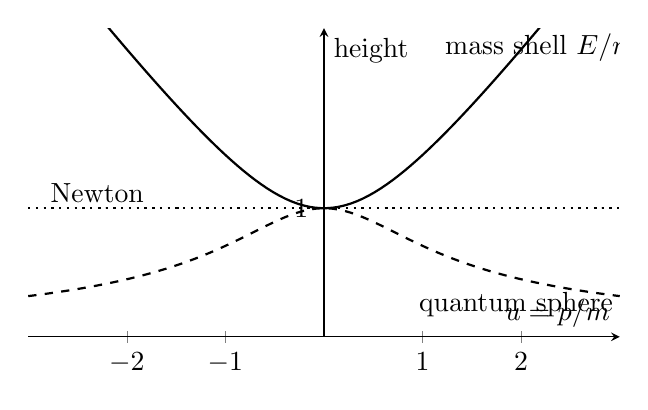
\begin{tikzpicture}
\begin{axis}[width=0.75\textwidth,height=5.5cm,axis lines=middle,xlabel={$u=p/m$},ylabel={height},xmin=-3,xmax=3,ymin=0,ymax=2.4,xtick={-2,-1,1,2},ytick={1},samples=100]
\addplot[black,thick,domain=-3:3] {sqrt(1+x^2)};
\addplot[black,dashed,thick,domain=-3:3] {1/sqrt(1+x^2)};
\addplot[black,dotted,thick,domain=-3:3] {1};
\node at (axis cs:2.2,2.25) {mass shell $E/m$};
\node at (axis cs:2.3,0.25) {quantum sphere $m/E$};
\node at (axis cs:-2.3,1.12) {Newton};
\end{axis}
\end{tikzpicture}
\caption{The mass shell (solid) and the quantum sphere (dashed) over the same proper velocity $u$. They touch at rest with the Newtonian plane (dotted) and bend in opposite directions; their heights are reciprocal.}
\label{fig:recip}
\end{figure}

So the two surfaces are mirror images through the plane of Newtonian physics. Both pass through the rest point with zero slope, the shell bends up with second derivative $+1$ and the sphere bends down with $-1$. They belong to a single family $X_0=\sqrt{1-\kappa X^2}$, all tangent at the rest point, with second derivative $-\kappa$: the sphere is $\kappa=1$, the shell $\kappa=-1$, and Newton is $\kappa=0$ (\lean{cayley\_klein}). Restoring units, $\kappa=\pm1/c^2$.

\section{The metric of the quantum sphere}

The quantum sphere is not just a picture; it has a metric, induced from $S^3$, and it is related to the hyperbolic metric of the shell by a simple factor.

\begin{proposition}\proved\label{prop:pullback}
The metric of $S^3$ pulled back by $Q$ is
\[
\partial_iQ\cdot\partial_jQ=\frac{\delta_{ij}}{E^2}-\frac{p_ip_j}{E^4},
\]
and it equals the metric of the mass shell divided by $E^2$: the quantum hemisphere is conformal to hyperbolic space.
\end{proposition}
\noindent In the repository: \lean{pullback\_metric}, \lean{conformal}, \lean{metric\_pullback}.

The conformal factor has a direct consequence for areas. A cap of the hemisphere of polar radius $\chi_0=\operatorname{gd}\eta_0$ has area $2\pi(1-m/E_0)$, and the corresponding disc on the shell has area $mE_0$ times larger (\lean{area\_Q}, \lean{area\_ratio}). As $E_0\to\infty$ the hemisphere's area tends to the finite value $2\pi$ while the shell's grows without bound. Infinite momentum space has been folded into a finite, round region, and it is round in the way that rotations are round.

\begin{asidebox}{A thought to carry forward}
In Chapter~4 the sphere of rotations and the hyperboloid of boosts were the real and imaginary slices of one complex quadric. Here the same pair appears in physics: the hyperboloid is where the particle's motion lives, and the hemisphere is where its quantum state lives. The cap of the dumbbell will be a round $S^3$, and the neck will contain a hyperbolic plane.
\end{asidebox}

\begin{standsbox}
The map $Q$ and its pullback metric are elementary, and the relation to the Dirac Hamiltonian is standard. The organisation of shell, sphere and Newtonian plane into one family tangent at rest, and the bookkeeping of areas, are presentations developed for this book; they are checked but not claimed as research results.
\end{standsbox}

\section*{Exercises}
\begin{exercise}Show that $Q(\mathbf p)$ is a unit quaternion with positive real part. \emph{Answer:} \lean{qD\_unit}, \lean{qD\_upper}.\end{exercise}
\begin{exercise}Show that $Q$ is injective. \emph{Answer:} \lean{qmap\_inj}.\end{exercise}
\begin{exercise}Show that $wX_0=1$. \emph{Answer:} \lean{qh\_reciprocal}.\end{exercise}
\begin{exercise}Compute the second derivatives of $\sqrt{1+u^2}$ and $1/\sqrt{1+u^2}$ at $u=0$. \emph{Answer:} \lean{curv\_H\_Q}, \lean{cayley\_klein}.\end{exercise}
\begin{exercise}Compute the area of a cap of the hemisphere. \emph{Answer:} \lean{area\_Q}.\end{exercise}
